\documentclass[10pt]{article}
\usepackage[utf8]{inputenc}
\usepackage[T1]{fontenc}
\usepackage{graphicx}
\usepackage[export]{adjustbox}
\graphicspath{ {./images/} }
\usepackage{amsmath}
\usepackage{amsfonts}
\usepackage{amssymb}
\usepackage[version=4]{mhchem}
\usepackage{stmaryrd}

\title{Optimizing Newton's Method for Machine Learning }

\author{}
\date{}


\begin{document}
\maketitle
\section*{Introduction}
In this project, we explored and tested the practical effectiveness of Newton's Method as an optimization technique within the machine learning context. We were interested in investigating whether this second-order method could be effectively adapted and optimized to train neural networks on a simple supervised learning problem: digit classification using the digits dataset.

To do this, we developed a feedforward neural network and trained it on the digits dataset provided by scikit-learn. What we focused our project on is the implementation of our own Newton's Method optimizer, including the computation of gradients and Hessians, and solving the resulting linear systems at each iteration. For this we had to learn the mathematical foundations of Newton's Method and numerical differentiation, matrix manipulation, and computational efficiency.

Once we had a working implementation, we compared the performance of our Newton-based optimizer against two widely used optimization algorithms in machine learning: Stochastic Gradient Descent (SGD) and ADAM. By training and testing the model with the different optimizers, we observed that our optimizer was able to reduce training error over time and showed the convergence properties we were looking for. However, despite these results we achieved, our optimizer did not reach the level of performance achieved by ADAM or SGD in terms of accuracy, and also our optimizer took a lot more time to train when compared to these others.

This outcome shows that using Newton's Method for machine learning is possible, but might not be ideal. While it also uses the second-order derivative to converge, it is made worse because of the computational complexity of calculating the Hessian matrix-especially in higher dimensions. However, this project can serve as insight on the potential challenges of incorporating second-order optimization techniques into neural network training.

\section*{Newton's method in optimization}
Missing text goes here

\section*{Network model}
We used Tensorflow with Keras to build our network model. The dataset we used was "Pen-Based Recognition of Handwritten Digits" which consists of 8x8 images of handwritten digits. Our network consists of an input layer of 64 neurons (one for each pixel), a hidden layer of 32 neurons with ReLU as their activation function, and an output layer of 10 neurons (one for each digit) with softmax as the activation. For the ADAM and SGD optimizers, we used Keras' built-in optimizers. We wrote the Newton's Method optimizer ourselves using Keras' automatic differentiation (through the use of Gradient Tapes and the built-in Jacobian method). The Adam and SGD models were trained using Tensorflow's fit method, and the Newton's method model was trained using our own train function, as there was no pre-existing function to do this. When analyzing the results, it is important to take into account that the networks using ADAM and SGD will have a slight advantage over the network using our custom Newton's Method optimizer, as the code for these two optimizers was written and optimized by Tensorflow developers over many years.

\section*{Results and conclusions}
We trained and evaluated the model's performance over the course of 50 training epochs, comparing our Newton's Method optimizer with ADAM and Stochastic Gradient Descent (SGD). The results, shown in the training loss and accuracy plots, reveal several important insights into the strengths and limitations of each approach.\\
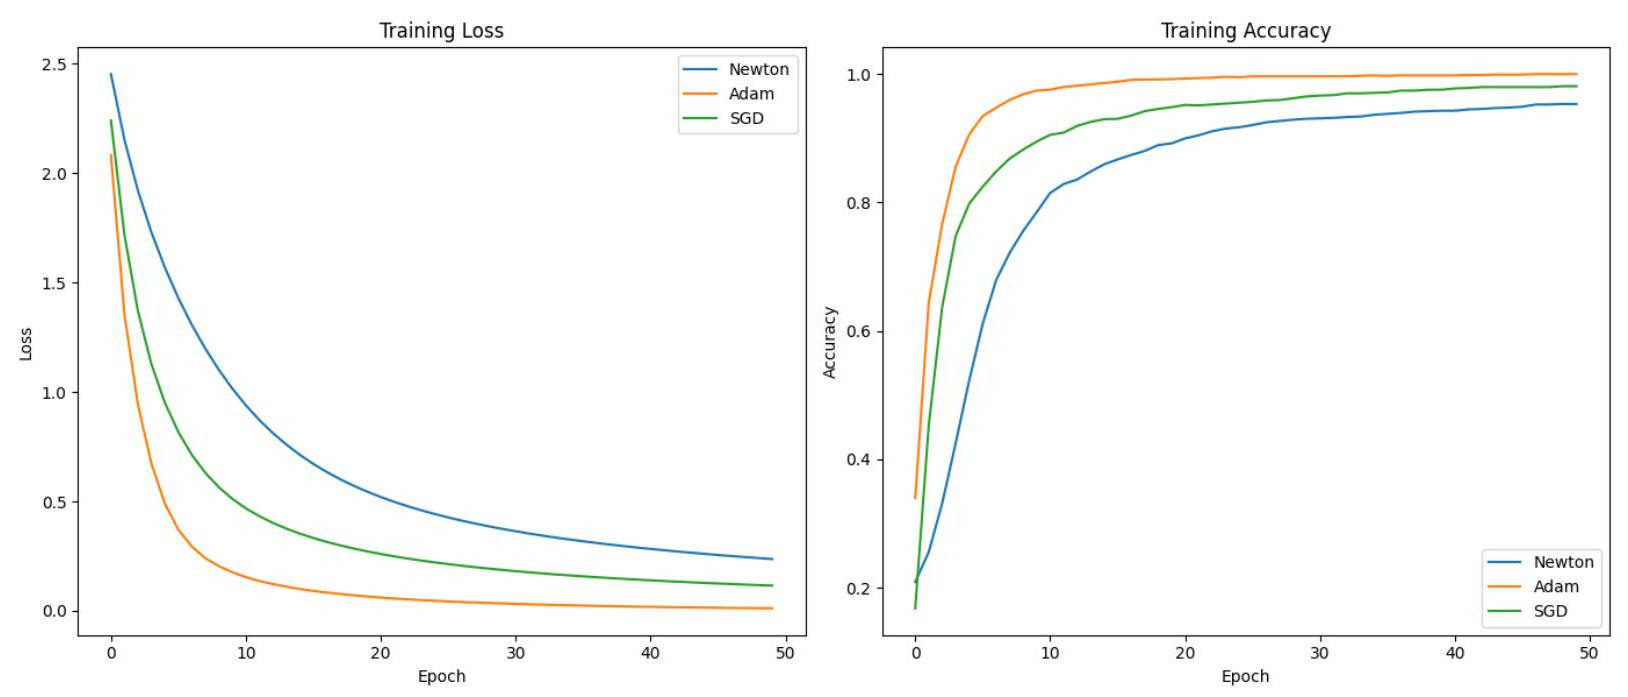
\includegraphics[max width=\textwidth, center]{2025_04_08_c5129b05008e68f8b3cdg-2}

From the training loss graph, it can be seen that ADAM achieved the fastest and most stable convergence, reducing the loss to near zero within the first 20 epochs. SGD also performed well, it still converged slower than ADAM but still significantly reduced the loss over the epochs. Newton's Method, while improving the loss steadily, underperformed when compared to both ADAM and SGD, as it showed a slower rate of convergence.

Similarly, the training accuracy graph highlights that ADAM quickly pushed the model to over $95 \%$ accuracy, with SGD really close to it. Newton's Method displayed a more gradual improvement in accuracy, reaching around $93 \%$ by the end of training. While this is a very good result, it always performed worse than the other two optimizers.

These results suggest that while Newton's Method has theoretical advantages, such as quadratic convergence near the optimal values, its practical application in training neural networks is limited by the computational cost of its operations and because the initial conditions affect it greatly. The cost of calculating the Hessian matrix at each step likely contributed to its slower performance.

Despite this, our implementation demonstrated that Newton's Method is capable of reducing error and improving accuracy just by calculating the gradient and the hessian, and without using any adaptive strategies like ADAM.

In conclusion, our project shows that Newton's Method works as an optimization algorithm in machine learning but may not be ideal, especially when compared with modern first-order optimizers for large-scale and real-time training tasks, as these take much less time than our custom Newton's method optimizer.

\section*{Extensions and Applications}
Once again, the performance of the Newton's Method optimizer was heavily impacted by the fact that we wrote the optimizer ourselves, rather than using a pre-written optimizer. A direct extension on our project would be to optimize our optimizer. One such way to do this is to code it in a faster language like $\mathrm{C} / \mathrm{C}++$ and to improve on the calculation of the hessian.

Other extensions include using Newton's Method in other machine learning contexts, such as non-classification neural networks such as regression, or even in unsupervised or reinforcement learning. Another possible extension is the use of other optimization algorithms to train networks, such as derivative-free algorithms. We could also use Newton's Method in other contexts, such as in symbolic calculators.

\section*{References}

\end{document}